\question Observa el esquema de una cancha de basquetbol de la figura \ref{fig:17.8}. Nota que las medidas están en pulgadas y pies.

\begin{parts}
    \part[5] Calcula el área de una de las regiones de tiros de falta (foul) formada por un rectángulo y un semicírculo.
    \part[5] Determina las áreas de los círculos centrales.
    \part[5] Calcula el área de las dos regiones de tres puntos.
\end{parts}

\begin{figure}[H]
    \centering
    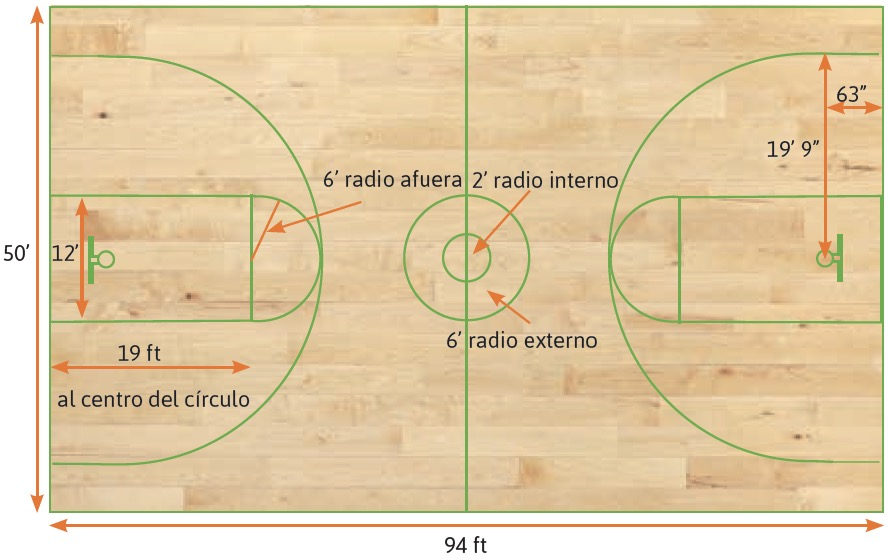
\includegraphics[width=0.8\linewidth]{17.8.jpg}
    \captionof{figure}{Cancha de basquetbol con medidas.}
    \label{fig:17.8}
\end{figure}